

\documentclass[conference]{IEEEtran}

\usepackage[utf8]{inputenc}
\usepackage[pdftex]{graphicx}
%\usepackage{unicode-math}
%\usepackage{mathtools}
\usepackage{amsmath}

\usepackage{filecontents,pgfplots}
\hyphenation{op-tical net-works semi-conduc-tor}


\begin{document}

\renewcommand{\abstractname}{Resumo}
\renewcommand{\refname}{REFERÊNCIAS}
\renewcommand{\tablename}{TABELA}


\title{Análise de Complexidade e Experimental de Algoritmos de Ordenação}


% author names and affiliations
% use a multiple column layout for up to three different
% affiliations
%\author{\IEEEauthorblockN{Bruno Santos de Lima\\Leandro Ungari Cayres}
%\IEEEauthorblockA{Faculdade de Ciências e Tecnologia\\
%Universidade Estadual Paulista\\
%Presidente Prudente, Brasil\\
%\textit{leandroungari@gmail.com}}
%}

\author{ 
 Bruno Santos de Lima\\ 
 \IEEEauthorblockA{Faculdade de Ciências e Tecnologia\\
Universidade Estadual Paulista\\
Presidente Prudente, Brasil \\
 \textit{brunoslima4@gmail.com}
} 
 \and 
 Leandro Ungari Cayres\\ 
 \IEEEauthorblockA{Faculdade de Ciências e Tecnologia\\
Universidade Estadual Paulista\\
Presidente Prudente, Brasil \\
 \textit{leandroungari@gmail.com} 
}
} 



% make the title area
\maketitle

% As a general rule, do not put math, special symbols or citations
% in the abstract
%\begin{abstract}
 

%~\\Palavras-chave: ordenação, análise assintótica e análise experimental.

%\end{abstract}


\IEEEpeerreviewmaketitle


\section{Introdução}

Diversas aplicações da atualidade envolvem um grande volume de dados, desde aplicações comerciais simples a grande aplicações científicas, todas estão nesse contexto. A organização estrutural de conjunto de dados, além de prover melhor usabilidade, também otimiza tempo e o consumo de recursos, tanto de processamento quanto de memória para a execução.

Neste contexto, este trabalho apresenta uma análise dos principais algoritmos de ordenação, o qual está dividido nas seguintes seções: na Seção 2, são apresentados os algoritmos de ordenação utilizados, indicando a abordagem utilizada no processo juntamente com a sua respectiva análise assintótica. Na Seção 3, são apresentados os estudos comparativos analisando a variações dos conjunto de dados de entrada e abordagens utilizadas na ordenação. Por fim, na Seção 4, são apresentadas as considerações finais do estudo.


\section{Algoritmos de Ordenação}


\subsection{Algoritmos baseados em Troca}


\subsubsection{Bubble Sort}

O presente algoritmo utilizada a abordagem de troca, através da permutação de elementos vizinhos, seguindo a ideia de densidade dos elementos, em que pode-se optar por varrer o arranjo levando o maior elemento (mais pesado) ao fim do vetor, ou conduzir o menor elemento (mais leve) ao início desse. Esse passo (uma das duas opções excludentemente) é realizado sucessivamente para os subvetores não ordenados remanescentes até que o vetor esteja ordenado como um todo.

A abordagem original prevê que todos os elementos adjacentes sejam comparados através de $n - 1$ iterações, porém é possível que o arranjo esteja ordenado sem que sejam necessárias todos esses ciclos. De modo a prevenir operações desnecessárias, algumas abordagens utilizam-se de \textit{flags} para a detecção de trocas, caso a última iteração tenha ao menos uma ocorrência, há necessidade de pelo menos mais uma iteração, em caso negativo, o processo pode ser encerrado.

\begin{figure}

  \centering
    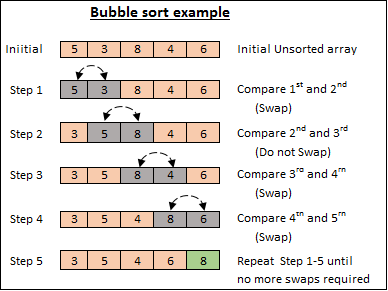
\includegraphics[width=0.4\textwidth]{images/bubble.png}
    \label{image:modelo}
    \caption{Modelo de comparação de elementos adjacentes.}
\end{figure}

A Figura~\ref{image:modelo} apresenta a abordagem de ordenação utilizada pelo algoritmo referido.\\

Complexidade:
\begin{itemize}
\item \textbf{Melhor caso:} $O (n)$, para vetor crescente somente na implementação com melhoria.
\item \textbf{Caso médio:} $O (n^2)$.
\item \textbf{Pior caso:} $O (n^2)$, para vetor decrescente e aleatório.
\end{itemize}

~\\
\subsubsection{Quick Sort}

O algoritmo foi proposto por C.A.R. Hoare em 1962, tem como estratégia a divisão do arranjo original em partições a partir da determinação de um pivô. Para qualquer abordagem de escolha do pivô, em cada partição busca-se encontrar os elementos maiores que o pivô a partir do início e os menores a partir do fim do arranjo, os quais são trocados de posição aos pares, de modo a ordenar a partição, se necessário também através da quebra de subpartições.

Em relação a abordagem de escolha de pivô, há diversas técnicas que buscam explorar possíveis características dos elementos do arranjo. Dentre as principais, pode-se destacar a escolha do elemento inicial ou final do vetor, o uso de propriedades estatísticas como a média e mediana, entre outras. O principal objetivo de qualquer uma dessas estratégias é minimizar a ocorrência dos piores casos de recorrência, resultando em um comportamento assintótico quadrático.

Geralmente, os piores caso desse algoritmo consistem na escolha de pivô como elemento mínimo ou máximo, para entradas de dados crescentes e decrescentes.\\

Complexidade:
\begin{itemize}
\item \textbf{Melhor caso:} $O (nlog n)$.
\item \textbf{Caso médio:} $O (nlog n)$.
\item \textbf{Pior caso:} $O (n^2)$, em geral para o pivô mínimo e máximo.
\end{itemize}


~\\
\subsection{Algoritmos baseados em Inserção}

\subsubsection{Insertion Sort}

A estratégia de ordenação por inserção consiste em um dos métodos mais simples, sendo extremamente eficiente em conjuntos pequenos, com estratégia de percorrer o esquerdo da esquerda para a direita deixando os elementos ordenados  à esquerda. Uma situação cotidiana que aplica a abordagem referida é a inserção de cartas na mão de um jogador, seguindo a estrutura de dados deque.\\

Complexidade:
\begin{itemize}
\item \textbf{Melhor caso:} $O (n)$, para arranjo crescente.
\item \textbf{Caso médio:} $O (n^2)$.
\item \textbf{Pior caso:} $O (n^2)$.
\end{itemize}

~\\
\subsubsection{Shell Sort}

O algoritmo Shell Sort foi proposto por Donald Shell em 1959, consistindo em um dos métodos de ordenação mais eficientes dentre os modelos quadráticos, baseando-se no Insertion Sort, a partir de comparações com elementos não adjacentes, desse modo, facilitando o deslocamento dos menores elementos para o início do vetor através do uso de saltos regressivos de tamanho.

O grande diferencial desse método é a utilização dos saltos, porém não existe uma abordagem única para o cálculo do tamanho dos saltos, consistindo em um fator determinante na mensuração da complexidade assintótica. Dentre os principais modelos têm-se o $n$ primeiros múltiplos de um fator ou combinação de fatores (ex. $2^p3^q$) ou os $n$ primeiros números primos.

\begin{figure}

  \centering
    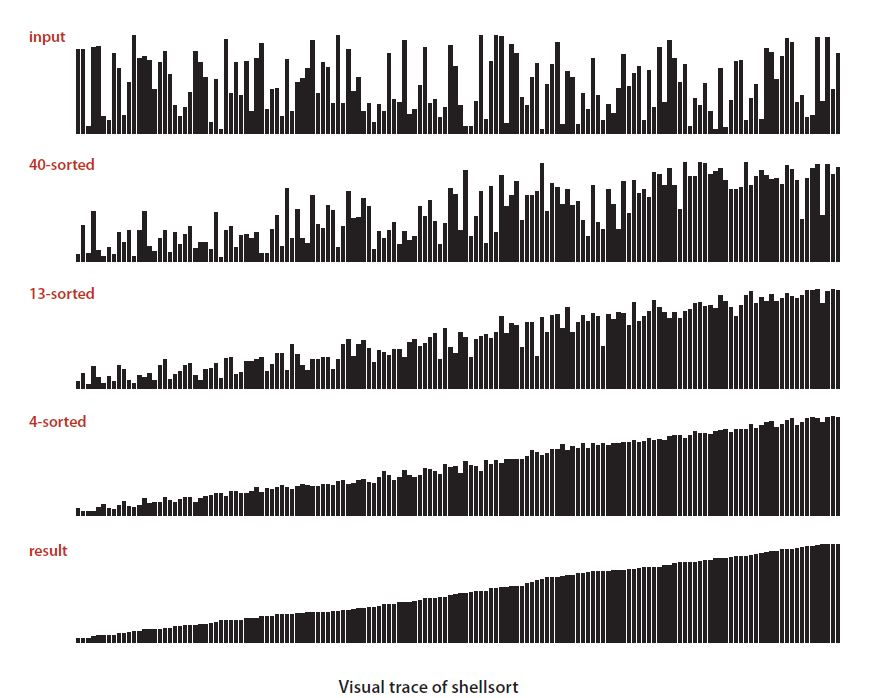
\includegraphics[width=0.4\textwidth]{images/shell.jpg}
    \label{image:shell}
     \caption{Modelo de partições com elementos distantes em diferentes tamanhos.}
\end{figure}

A Figura~\ref{image:shell} apresenta a ordenação das partições de elementos distantes, com saltos de tamanho 40, 13 e 4 respectivamente, partindo do arranjo inicial e alcançando o conjunto ordenado.\\

Complexidade:
\begin{itemize}
\item \textbf{Caso médio:} $O (n^{3/2})$
\end{itemize}
~\\
\subsection{Algoritmos baseados em Seleção}


\subsubsection{Selection Sort}

O algoritmo Selection Sort, trata-se modelo mais básico de algoritmo de ordenação, utilizada muitas em ambientes naturais e é mais intuitivo para os seres humanos, pois se utiliza da abordagem de força bruta, sem aproveitar nenhuma peculiaridade do conjunto de dados ou vantagem que possa ser tomada. Sua estratégia consiste em percorrer todo o arranjo $n$, comparando todos os elementos de forma a encontrar o menor, em seguida, o segundo menor e assim por diante, de modo a organizar todo o conjunto.

O grande destaque para esse algoritmo, dentro do contexto das abordagens quadráticas, consiste no reduzido número de trocas, que no máximo ocorre $n$ vezes.\\

Complexidade:
\begin{itemize}
\item \textbf{Caso médio:} $O (n^2)$, de modo invariante.
\end{itemize}

~\\
\subsubsection{Heap Sort}

O algoritmo Heap Sort, proposto por J.W.J. Williams em 1964, possui uma das implementações mais sofisticadas baseando-se em uma fila de prioridades, através da utilização de um vetor para a representação de uma árvore binária, caracterizando como um dos algoritmos mais estáveis de ordenação, independentemente do modelo de dados de entrada. 

\begin{figure}
  
  \centering
    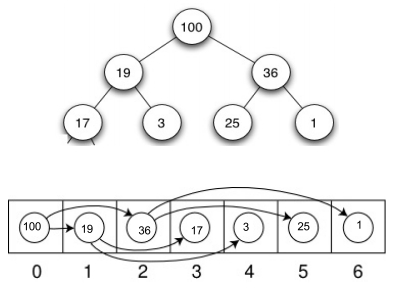
\includegraphics[width=0.4\textwidth]{images/heapsort.jpg}
    \label{image:arvore}
  \caption{Equivalência entre a árvore e arranjo.}
\end{figure}

A Figura~\ref{image:arvore} apresenta o processo de equivalência entre a estrutura de dados Heap na forma de árvore e arranjo.

O algoritmo consiste na construção de um \textit{max heap} (cuja principal propriedade consiste em que sempre o elemento raiz é maior que seus filhos, para todas as sub-árvores possíveis), em seguida, aplica-se a troca do primeiro elemento pelo último para todos os elementos do conjunto (equivalente a remover todos os elementos do arranjo), e posteriormente, rearranjar a estrutura para cada elemento, desse modo é obtido um vetor ordenado de modo crescente ao termino do processo.\\

Complexidade:
\begin{itemize}
\item \textbf{Caso médio:} $O (nlog n)$, de modo invariante.
\end{itemize}

~\\
\subsection{Algoritmos baseados em Intercalação}

\subsubsection{Merge Sort}

Este algoritmo utiliza o princípio de divisão e conquista, de modo a quebrar um problema complexo em sub-problemas, até o caso base (restante um ou dois elementos no sub-vetor), de modo que seja possível ordená-los. A partir da garantia de que todos os sub-arranjos estão ordenadas, inicia-se o processo de combinação entre eles, de modo recursivo, até alcançar o problema original, de modo ordenado.

As posições situações de ocorrência são as seguintes:
\begin{itemize}
\item em seu seu melhor caso nunca é necessário realizar trocas após comparações;
\item o caso médio ocorre quando nem sempre é necessário realizar trocas após comparações;
\item por fim, o pior caso ocorre quando sempre é necessário realizar trocas após comparações.
\end{itemize}~\\

Contudo, de modo invariável, todos os casos tem a mesma complexidade assintótica. Adicionalmente, vale-se destacar que diferentemente dos demais algoritmos que não se utilizam de memória adicional, o algoritmo Merge Sort tem complexidade espacial de tamanho $n$, que em dadas situações, deve ser levada em consideração.

\begin{figure}
  
  \centering
    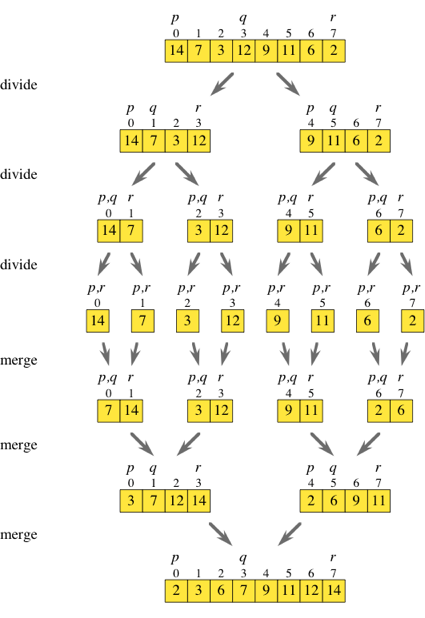
\includegraphics[width=0.4\textwidth]{images/merge.png}
    \label{image:merge}
  \caption{Abordagem de divisão e conquista do algoritmo.}
\end{figure}

A Figura~\ref{image:merge} apresenta o processo de divisão e conquista utilizado no algoritmo.\\

Complexidade:
\begin{itemize}
\item \textbf{Caso médio:} $O (nlog n)$, de modo invariante.
\end{itemize}

~\\
%==================================
\section{Análise Experimental}

De modo a prover uma análise experimental em relação aos algoritmos, foram conduzidos estudos com diferentes tamanhos de entrada, cujas dimensões foram: 10, 100, 1 000, 10 000, 100 000, 500 000 e 1 000 0000 de elementos, em que para todos os casos foram utilizados como teste um vetor crescente, decrescente e elementos dispersos pelo vetor de forma aleatória (vale ressaltar que para este último foi utilizado um arquivo que armazena os elementos, para que esta sequência aleatória seja sempre a mesma para execução em todos os algoritmos). Todos os casos foram avaliados em relação ao tempo medido em milissegundos (ms) e possuíram três execuções, em que foi escolhido o caso mediano. 

Para a realização da análise experimental foi utilizado um notebook com as seguintes especificações: processador Intel Core i7-7700HQ CPU @ 2.80 GHz de 4 núcleos físicos e 8 threads, com memória cache L1 de 256 KB, L2 de 1 MB, L3 de 6 MB e memória RAM de 8 GB DDR4.


\subsection{Modelos de entrada de dados}
As análises experimentais a seguir realizam uma comparação entre todos os métodos de ordenação para cada caso de entrada de dados específico, sendo ordenado de modo crescente, decrescente e aleatório.
~\\
\subsubsection{Entrada crescente}

Inicialmente, através da Figura~\ref{image: crescente}, pode-se observar que as estratégias de ordenação dos algoritmos \textit{Bubble Sort Clássico}, \textit{Selection Sort} e o \textit{Quick Sort} com pivô inicial apresentaram desempenhos inferiores aos demais, principalmente em relação a esse último, que a partir de uma dada grandeza de entrada superou os outros dois, desse modo é possível notar o impacto que a quebra inadequada de partições pode ocasionar.

Em relação aos outros algoritmos, esses apresentaram melhores desempenhos, assemelhando-se a algoritmos lineares, devido a presença de estratégias que reduzem o número de operações sobre os elementos, com destaque ao \textit{Insertion Sort}, um algoritmo inicialmente quadrático, torna-se o mais eficiente entre os analisados.

\begin{figure}


\centering
\pgfplotstableread{plots/crescente.dat}{\pistonkinetics}
\begin{tikzpicture}[scale=1]
\begin{axis}[legend style={at={(0.5,-0.1)},anchor=north}]
\addplot [black,very thick] table [x={n}, y={bubble-class}] {\pistonkinetics};
\addlegendentry{Bubble Sort}
\addplot [red,very thick] table [x={n}, y={bubble-adv}] {\pistonkinetics};
\addlegendentry{Bubble Sort Avançado}
\addplot [blue,very thick] table [x={n}, y={quick-inicial}] {\pistonkinetics};
\addlegendentry{Quick Sort Inicial}
\addplot [green,very thick] table [x={n}, y={quick-central}] {\pistonkinetics};
\addlegendentry{Quick Sort Central}
\addplot [yellow,very thick] table [x={n}, y={insertion}] {\pistonkinetics};
\addlegendentry{Insertion Sort}
\addplot [gray,very thick] table [x={n}, y={shell}] {\pistonkinetics};
\addlegendentry{Shell Sort}
\addplot [brown,very thick] table [x={n}, y={selection}] {\pistonkinetics};
\addlegendentry{Selection Sort}
\addplot [pink,very thick] table [x={n}, y={merge}] {\pistonkinetics};
\addlegendentry{Merge Sort}
\addplot [orange,very thick] table [x={n}, y={heap}] {\pistonkinetics};
\addlegendentry{Heap Sort}
\end{axis}
\end{tikzpicture}
\caption{Comparativo de execução para entrada crescente.}
\label{image: crescente}
\end{figure}

~\\
\subsubsection{Entrada decrescente}

Através do gráfico representado pela Figura~\ref{image: decrescente}, permite-se observar a formação de três conjuntos de desempenho de algoritmos. No primeiro conjunto, pior desempenho, composto pelas duas implementações do \textit{Bubble Sort}, é possível caracterizar o pior caso de ambos, de modo que nenhuma estratégia adicional para otimização tem efeito no desempenho. 

Em seguida, no segundo conjunto, enquadram-se os algoritmos \textit{Insertion Sort}, \textit{Quick Sort} com pivô inicial e \textit{Selection Sort}, com um comportamento próximo de quadrático, porém com um menor número de operações de comparação entre detrimento ao primeiro grupo.

O último caso dessa análise estão os algoritmos \textit{Heap Sort}, \textit{Merge Sort}, \textit{Shell Sort} e \textit{Quick Sort} com pivô central, demonstrando que em dadas situações um algoritmo baseado em inserção pode se equiparar a implementações mais sofisticadas.

\begin{figure}
\centering
\pgfplotstableread{plots/decrescente.dat}{\pistonkinetics}
\begin{tikzpicture}[scale=1]
\begin{axis}[legend style={at={(0.5,-0.1)},anchor=north}]
\addplot [black,very thick] table [x={n}, y={bubble-class}] {\pistonkinetics};
\addlegendentry{Bubble Sort}
\addplot [red,very thick] table [x={n}, y={bubble-adv}] {\pistonkinetics};
\addlegendentry{Bubble Sort Avançado}
\addplot [blue,very thick] table [x={n}, y={quick-inicial}] {\pistonkinetics};
\addlegendentry{Quick Sort Inicial}
\addplot [green,very thick] table [x={n}, y={quick-central}] {\pistonkinetics};
\addlegendentry{Quick Sort Central}
\addplot [yellow,very thick] table [x={n}, y={insertion}] {\pistonkinetics};
\addlegendentry{Insertion Sort}
\addplot [gray,very thick] table [x={n}, y={shell}] {\pistonkinetics};
\addlegendentry{Shell Sort}
\addplot [brown,very thick] table [x={n}, y={selection}] {\pistonkinetics};
\addlegendentry{Selection Sort}
\addplot [pink,very thick] table [x={n}, y={merge}] {\pistonkinetics};
\addlegendentry{Merge Sort}
\addplot [orange,very thick] table [x={n}, y={heap}] {\pistonkinetics};
\addlegendentry{Heap Sort}
\end{axis}
\end{tikzpicture}

\caption{Comparativo de execução para entrada decrescente.}
\label{image: decrescente}
\end{figure}

~\\
\subsubsection{Entrada aleatória}


O experimento revelou que para esta organização do conjunto os algoritmos Heap Sort, Merge Sort, Shell e Quick Sort para ambas implementações tiveram um desempenho considerado superior com relação aos demais. Os algoritmos de pior rendimento consistem nas duas implementações do Bubble Sort.

\begin{figure}

\centering
\pgfplotstableread{plots/aleatorio.dat}{\pistonkinetics}
\begin{tikzpicture}[scale=1]
\begin{axis}[legend style={at={(0.5,-0.1)}, anchor=north}]
\addplot [black,very thick] table [x={n}, y={bubble-class}] {\pistonkinetics};
\addlegendentry{Bubble Sort}
\addplot [red,very thick] table [x={n}, y={bubble-adv}] {\pistonkinetics};
\addlegendentry{Bubble Sort Avançado}
\addplot [blue,very thick] table [x={n}, y={quick-inicial}] {\pistonkinetics};
\addlegendentry{Quick Sort Inicial}
\addplot [green,very thick] table [x={n}, y={quick-central}] {\pistonkinetics};
\addlegendentry{Quick Sort Central}
\addplot [yellow,very thick] table [x={n}, y={insertion}] {\pistonkinetics};
\addlegendentry{Insertion Sort}
\addplot [gray,very thick] table [x={n}, y={shell}] {\pistonkinetics};
\addlegendentry{Shell Sort}
\addplot [brown,very thick] table [x={n}, y={selection}] {\pistonkinetics};
\addlegendentry{Selection Sort}
\addplot [pink,very thick] table [x={n}, y={merge}] {\pistonkinetics};
\addlegendentry{Merge Sort}
\addplot [orange,very thick] table [x={n}, y={heap}] {\pistonkinetics};
\addlegendentry{Heap Sort}
\end{axis}
\end{tikzpicture}

\caption{Comparativo de execução para entrada aleatório.}
\label{image: aleatoria}
\end{figure}

No último modelo de entrada de dados, representado pela Figura~\ref{image: aleatoria}, é possível observar que os algoritmos \textit{Heap Sort}, \textit{Merge Sort}, \textit{Shell Sort} e \textit{Quick Sort} obtiveram um desempenho com relação aos demais. De modo intermediário, os algoritmos \textit{Selection Sort} e \textit{Insertion} tiveram um desempenho pior se comparado ao primeiro grupo. 

Por fim, os algoritmos de pior rendimento consistem nas duas implementações do \textit{Bubble Sort}, em que deve-se destacar o elevadíssimo número de comparações como principal fator para o rendimento apresentado.


\subsection{Comparativo por algoritmo}

\subsubsection{Insertion Sort}

Por meio da Figura~\ref{image: graph-insertion}, permite observar que o algoritmo Insertion Sort consiste em um excelente opção para arranjos quase ordenados, pois caracteriza-se com complexidade quase linear, podendo ser muito útil em cenários que haja a construção do conjunto ordenado por demanda, indicado pela curva do arranjo crescente, contudo para os demais casos este torna-se próximo da complexidade quadrática, não consistindo na melhor escolha para tais situações.

\begin{figure}

\centering
\pgfplotstableread{plots/insertion-sort.dat}{\pistonkinetics}
\begin{tikzpicture}[scale=1]
\begin{axis}[legend style={at={(0.4,1)}}]
\addplot [black,very thick] table [x={n}, y={ale}] {\pistonkinetics};
\addlegendentry{Aleatório}
\addplot [red,very thick] table [x={n}, y={cresc}] {\pistonkinetics};
\addlegendentry{Crescente}
\addplot [blue,very thick] table [x={n}, y={desc}] {\pistonkinetics};
\addlegendentry{Decrescente}
\end{axis}
\end{tikzpicture}
\caption{Análise experimental do algoritmo Insertion Sort.}
\label{image: graph-insertion}
\end{figure}

\subsubsection{Shell Sort}
O gráfico representado pela Figura~\ref{image: graph-shell} demostra análise para diferentes casos de entrada do algoritmo Shell Sort, o qual apresenta um comportamento semelhante ao anterior, porém é capaz de lidar com tamanhos de conjunto de dados em um tempo muito mais inferior, enquanto o primeiro trabalha na grandeza de milhões de unidades de tempo, no caso milissegundos, o segundo trabalha na proporção dos milhares. 

Como a sua implementação consiste em uma melhoria da abordagem de inserção, a mesmas indicações de uso valem para este algoritmo.


\begin{figure}

\centering
\pgfplotstableread{plots/shell-sort.dat}{\pistonkinetics}
\begin{tikzpicture}[scale=1]
\begin{axis}[legend style={at={(0.4,1)}}]
\addplot [black,very thick] table [x={n}, y={ale}] {\pistonkinetics};
\addlegendentry{Aleatório}
\addplot [red,very thick] table [x={n}, y={cresc}] {\pistonkinetics};
\addlegendentry{Crescente}
\addplot [blue,very thick] table [x={n}, y={desc}] {\pistonkinetics};
\addlegendentry{Decrescente}
\end{axis}
\end{tikzpicture}
\caption{Análise experimental do algoritmo Shell Sort.}
\label{image: graph-shell}
\end{figure}

\subsubsection{Selection Sort}

Através do gráfico representado pela Figura~\ref{image: graph-selection}, pode-se concluir que o algoritmo de ordenação Selection Sort, apesar de ser indiferente quanto a organização prévia dos elementos pertencentes ao arranjo e ter uma das mais simples implementações, caracterizando-se como força-bruta, torna-se pior a medida que o número de elementos cresce, cuja curva se assemelha às quadráticas.

O principal e único destaque do algoritmo está relacionado ao número de trocas realizadas representado pelo gráfico na Figura !!!!!!!!!!!!!GRÁFICO DE TROCAS!!!!!!!!!!!!!!!
\begin{figure}


\centering
\pgfplotstableread{plots/selection-sort.dat}{\pistonkinetics}
\begin{tikzpicture}[scale=1]
\begin{axis}[legend style={at={(0.4,1)}}]
\addplot [black,very thick] table [x={n}, y={ale}] {\pistonkinetics};
\addlegendentry{Aleatório}
\addplot [red,very thick] table [x={n}, y={cresc}] {\pistonkinetics};
\addlegendentry{Crescente}
\addplot [blue,very thick] table [x={n}, y={desc}] {\pistonkinetics};
\addlegendentry{Decrescente}
\end{axis}
\end{tikzpicture}
\caption{Análise experimental do algoritmo Selection Sort.}
\label{image: graph-selection}
\end{figure}




\subsubsection{Heap Sort}

Por fim, o gráfico acima demonstra que o algoritmo Heap Sort mediante a uma implementação sofisticada promove resultados invariantes para todos os casos, sem o uso adicional de recursos.

\begin{figure}
\label{image: graph-heap}

\centering
\pgfplotstableread{plots/heap-sort.dat}{\pistonkinetics}
\begin{tikzpicture}[scale=1]
\begin{axis}[legend style={at={(0.4,1)}}]
\addplot [black,very thick] table [x={n}, y={ale}] {\pistonkinetics};
\addlegendentry{Aleatório}
\addplot [red,very thick] table [x={n}, y={cresc}] {\pistonkinetics};
\addlegendentry{Crescente}
\addplot [blue,very thick] table [x={n}, y={desc}] {\pistonkinetics};
\addlegendentry{Decrescente}
\end{axis}
\end{tikzpicture}
\caption{Análise experimental do algoritmo Heap Sort.}
\end{figure}

\subsubsection{Bubble Sort}

A análise experimental realizada com o método Bubble Sort em sua versão clássica revelou que independente do caso em que os elementos estão distribuídos no vetor, seja de modo aleatório, crescente ou decrescente o comportamento expresso no gráfico acima é semelhante, considerado de ordem quadrática, tendo para a organização inicial um vetor crescente seu desempenho foi levemente superior aos demais devido ao número reduzido de trocas entre elementos.

\begin{figure}
\label{image: graph-bubble}

\centering
\pgfplotstableread{plots/bubble-sort.dat}{\pistonkinetics}
\begin{tikzpicture}[scale=1]
\begin{axis}[legend style={at={(0.4,1)}}]
\addplot [black,very thick] table [x={n}, y={ale}] {\pistonkinetics};
\addlegendentry{Aleatório}
\addplot [red,very thick] table [x={n}, y={cresc}] {\pistonkinetics};
\addlegendentry{Crescente}
\addplot [blue,very thick] table [x={n}, y={desc}] {\pistonkinetics};
\addlegendentry{Decrescente}
\end{axis}
\end{tikzpicture}
\caption{Análise experimental do algoritmo Bubble Sort.}
\end{figure}

Os resultados da análise experimental revelaram que para o método de ordenação Bubble Sort com melhorias apresenta como seu melhor caso quando o vetor já está organizado de modo crescente tendo um desempenho linear, além disso tanto para conjuntos organizados de modo decrescente quanto para conjuntos organizados de forma aleatória temos um comportamento que se enquadra em seu pior caso com desempenho considerado quadrático, que é visivelmente observado em conjuntos de tamanho maior que cem mil.

\begin{figure}
\label{image: graph-bubble-adv}

\pgfplotstableread{plots/bubble-sort-adv.dat}{\pistonkinetics}
\begin{tikzpicture}[scale=1]
\begin{axis}[legend style={at={(0.4,1)}}]
\addplot [black,very thick] table [x={n}, y={ale}] {\pistonkinetics};
\addlegendentry{Aleatório}
\addplot [red,very thick] table [x={n}, y={cresc}] {\pistonkinetics};
\addlegendentry{Crescente}
\addplot [blue,very thick] table [x={n}, y={desc}] {\pistonkinetics};
\addlegendentry{Decrescente}
\end{axis}
\end{tikzpicture}
\caption{Análise experimental do algoritmo Bubble Sort Avançado.}
\end{figure}


\subsubsection{Quick Sort}
O experimento demonstrou que o algoritmo Quick Sort com pivô inicial tem um bom desempenho para um conjunto organizado em ordem aleatória, contudo para conjuntos em ordem crescente e decrescente o teste resultou em um baixo desempenho aumentando de forma considerável o tempo de execução.

\begin{figure}
\label{image: graph-quick-inicial}

\pgfplotstableread{plots/quick-sort-pivo-inicial.dat}{\pistonkinetics}
\begin{tikzpicture}[scale=1]
\begin{axis}[legend style={at={(0.4,1)}}]
\addplot [black,very thick] table [x={n}, y={ale}] {\pistonkinetics};
\addlegendentry{Aleatório}
\addplot [red,very thick] table [x={n}, y={cresc}] {\pistonkinetics};
\addlegendentry{Crescente}
\addplot [blue,very thick] table [x={n}, y={desc}] {\pistonkinetics};
\addlegendentry{Decrescente}
\end{axis}
\end{tikzpicture}
\caption{Análise experimental do algoritmo Quick Sort com pivô inicial.}
\end{figure}


Considerando a implementação do algoritmo Quick Sort utilizando um o pivô central é notório que nos casos em que o vetor está inicialmente ordenado de modo crescente e de modo decrescente o desempenho são semelhantes e melhores se comparados com um vetor com elementos dispostos aleatoriamente. 

\begin{figure}
\label{image: graph-quick-central}

\pgfplotstableread{plots/quick-sort-pivo-central.dat}{\pistonkinetics}
\begin{tikzpicture}[scale=1]
\begin{axis}[legend style={at={(0.4,1)}}]
\addplot [black,very thick] table [x={n}, y={ale}] {\pistonkinetics};
\addlegendentry{Aleatório}
\addplot [red,very thick] table [x={n}, y={cresc}] {\pistonkinetics};
\addlegendentry{Crescente}
\addplot [blue,very thick] table [x={n}, y={desc}] {\pistonkinetics};
\addlegendentry{Decrescente}

\end{axis}
\end{tikzpicture}
\caption{Análise experimental do algoritmo Quick Sort com pivô central.}
\end{figure}


\subsubsection{Merge Sort}

Em suma, a sua implementação baseada em divisão e conquista, permite um remanejamento dos elementos quase indiferente para os casos de conjunto crescente, decrescente e aleatório, colocando como um dos melhores algoritmos, apesar de seu maior consumo de memória.

\begin{figure}
\label{image: graph-merge}

\centering
\pgfplotstableread{plots/merge-sort.dat}{\pistonkinetics}
\begin{tikzpicture}[scale=1]
\begin{axis}[legend style={at={(0.4,1)}}]
\addplot [black,very thick] table [x={n}, y={ale}] {\pistonkinetics};
\addlegendentry{Aleatório}
\addplot [red,very thick] table [x={n}, y={cresc}] {\pistonkinetics};
\addlegendentry{Crescente}
\addplot [blue,very thick] table [x={n}, y={desc}] {\pistonkinetics};
\addlegendentry{Decrescente}
\end{axis}
\end{tikzpicture}
\caption{Análise experimental do algoritmo Merge Sort.}
\end{figure}

\subsection{Comparativo de abordagem}

\subsubsection{Abordagem de inserção}
\subsubsection{Abordagem de troca}
\subsubsection{Abordagem de seleção}



\section{Considerações Finais}



%\begin{thebibliography}{1}

%https://www.opentechguides.com/how-to/article/c/51/bubble-sort-c.html
%http://wiki.icmc.usp.br/images/b/b3/SCC501Cap4.pdf
%https://pt.khanacademy.org/computing/computer-science/algorithms/merge-sort/p/challenge-implement-merge-sort

%\bibitem{atlas}
%Programa das Nações Unidas para o Desenvolvimento (PNUD). \emph{Atlas do desenvolvimento humano do Brasil}. PNUD; 2003. Disponível em: http://www.pnud.org.br/atlas/

%\bibitem{senak}
%Sen AK. \emph{Desenvolvimento como liberdade}. São Paulo: Companhia das Letras; 2000.


%\end{thebibliography}




% that's all folks
\end{document}


